\chapter{Objekt-Semantik}

\begin{figure}[h]
  \centering
  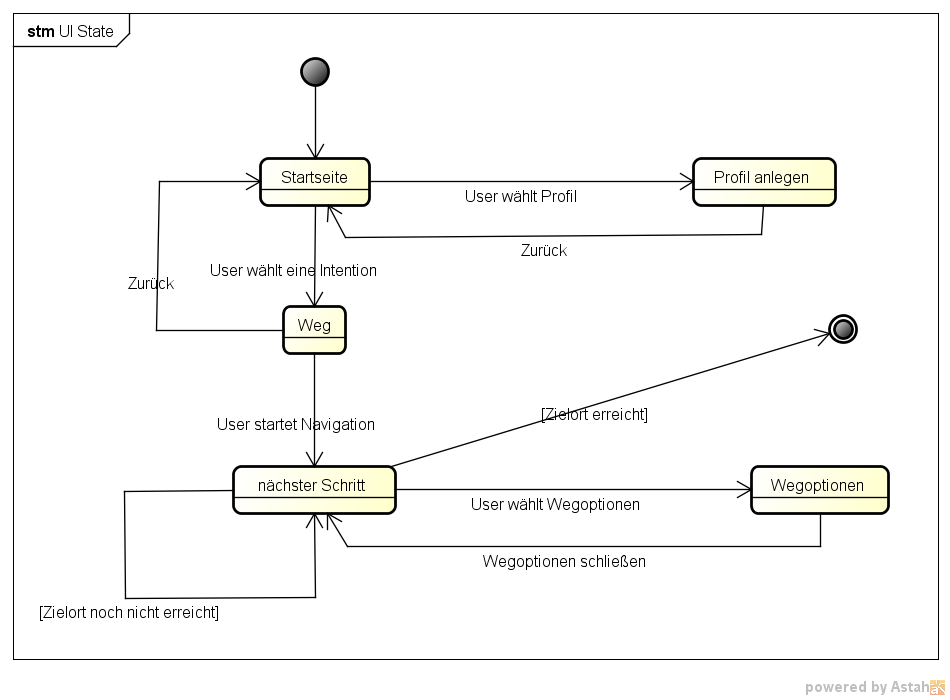
\includegraphics[width=\linewidth]{img/zustandsdiagramm.png}
  \caption{Zustandsdiagramm UI}
\label{fig:zustandsdiagramm}
\end{figure}

Das Zustandsdiagramm zeigt die verschiedenen Zustände und Folgezustände der
Nutzerschnittstelle. Es beschreibt welche Transitionen zwischen den Ansichten
und Modi der Nutzerschnittstelle möglich sind.

\begin{figure}[H]
  \centering
  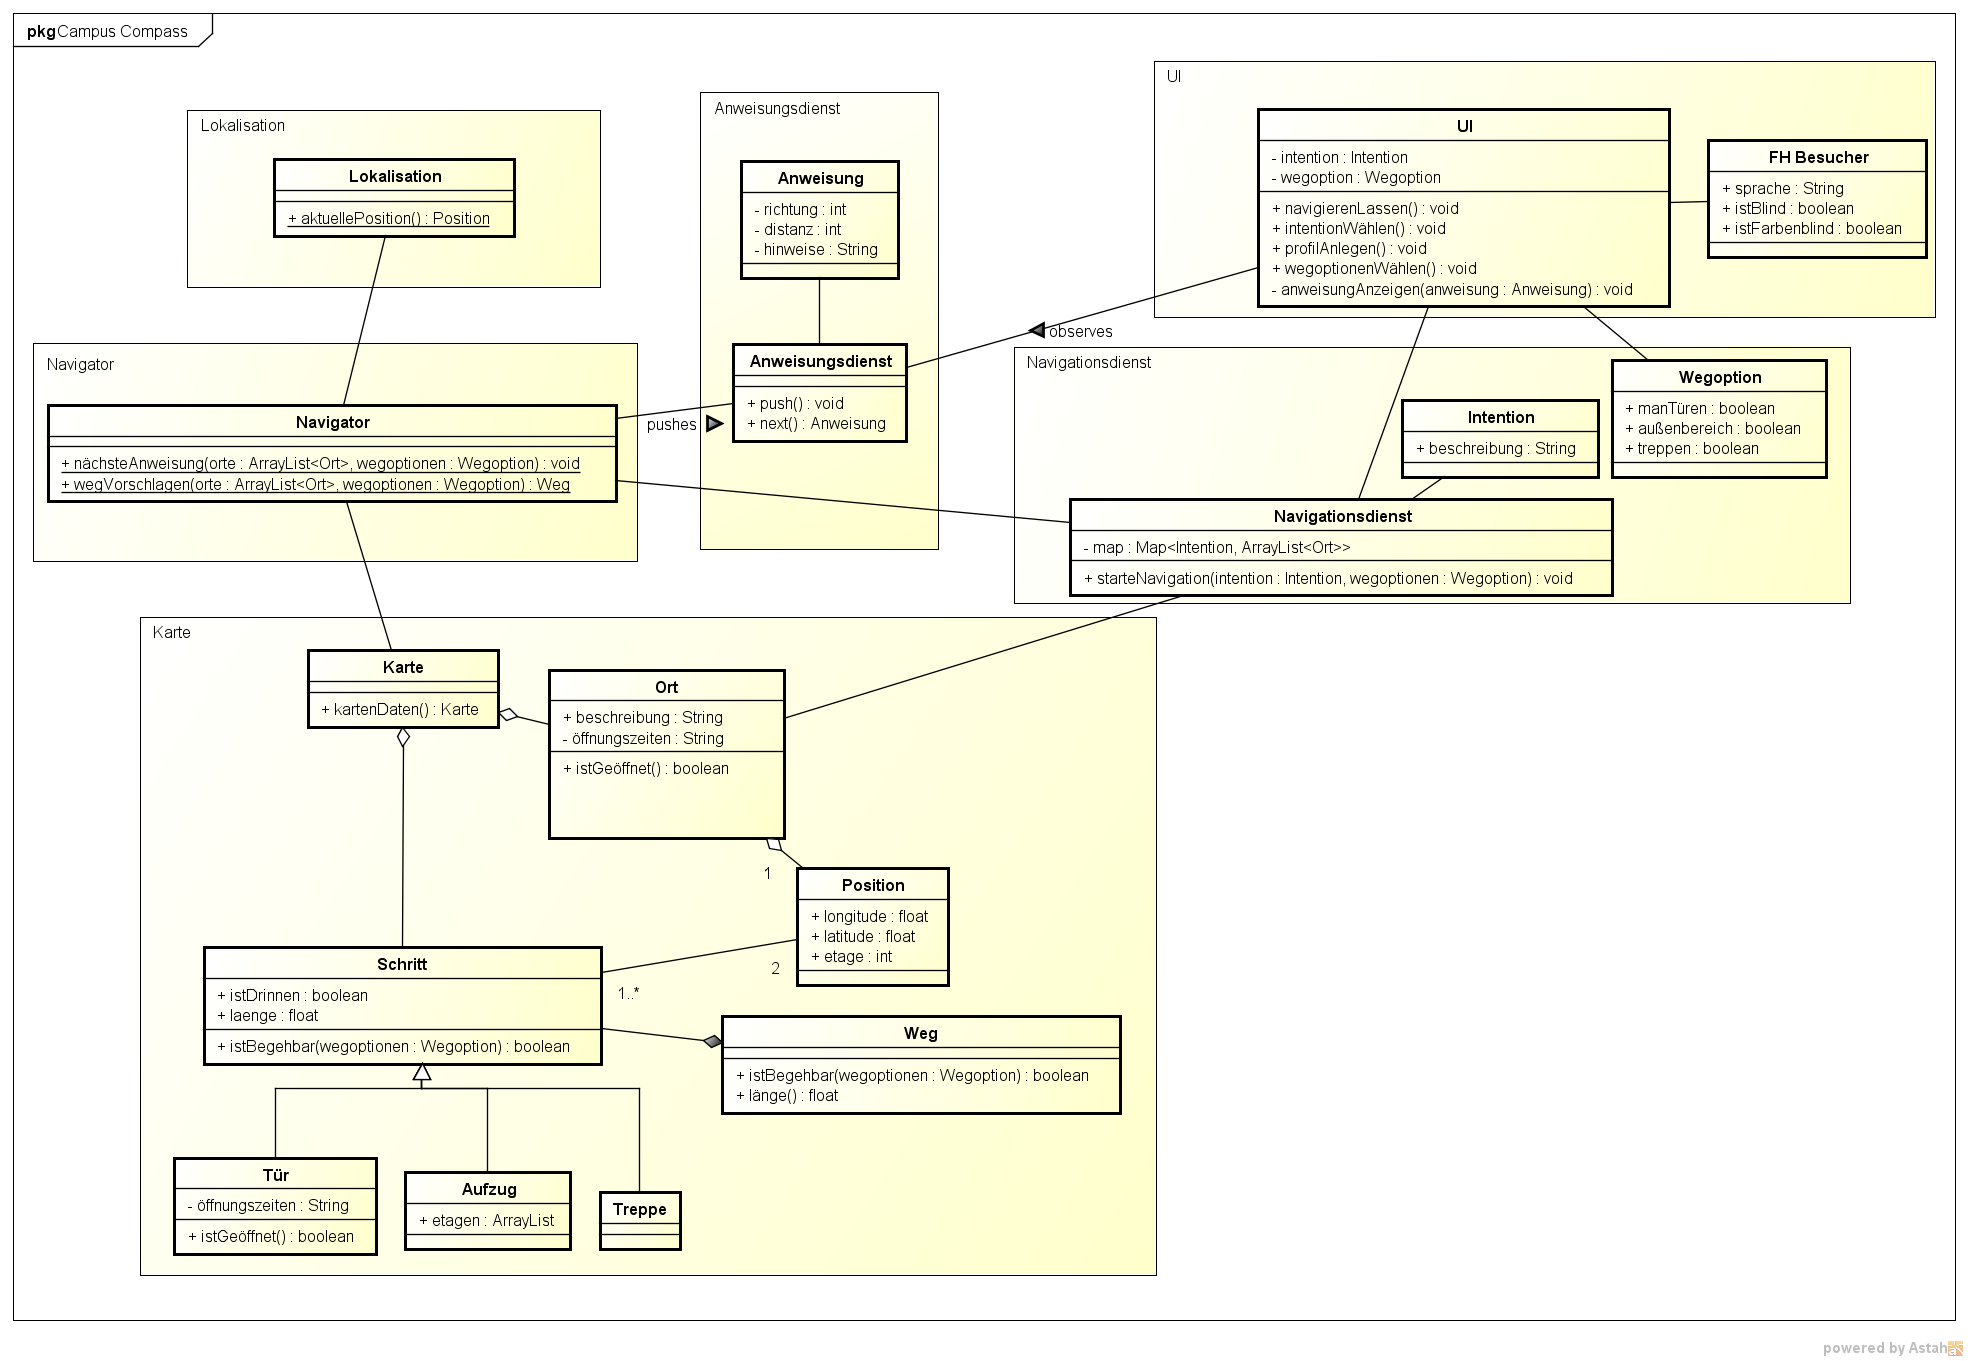
\includegraphics[width=\linewidth]{img/klassendiagramm.png}
  \caption{Klassendiagramm}
\label{fig:klassenDiagramm}
\end{figure}

Im Klassendiagramm zu sehen, sind die einzelnen Klassen des Systems,
zusammengefasst zu Komponenten. Diese finden sich später im Komponentendiagramm
wieder.

\noindent
Bemerkenswert ist hierbei der Anweisungsdienst, welcher dazu dient die UI vom
Navigator zu entkoppeln und ihm die direkte Kontrolle darüber entzieht, wann die
UI die von ihm gestellten Anweisungen an den Nutzer weitergibt.
